
\begin{table}[t]
\centering
\caption{Quantitative comparison on NeRF Synthetic and Shiny-Blender datasets. Ranking
(\colorbox{green!25}{\textbf{1st}}, \colorbox{orange!25}{2nd}, \colorbox{yellow!25}{3rd}) is
computed within the Fixed-Mesh block only, since these methods share our input mesh; the No-Mesh
and Flexible-Mesh blocks reconstruct their own geometry and are shown as context, not ranked
(numbers reported from RefGS~\citep{refgs}). The Fixed-Mesh rows (2DGS$^{*}$, DNR, and Ours) are
measured by us.}
\label{tab:main}
\resizebox{\linewidth}{!}{
\begin{tabular}{llcccccc}
\toprule
\multirow{2}{*}{\textbf{Constraint}} & \multirow{2}{*}{\textbf{Method}} & \multicolumn{3}{c}{NeRF Synthetic} & \multicolumn{3}{c}{Shiny-Blender} \\
\cmidrule(lr){3-5} \cmidrule(lr){6-8}
& & PSNR$\uparrow$ & SSIM$\uparrow$ & LPIPS$\downarrow$ & PSNR$\uparrow$ & SSIM$\uparrow$ & LPIPS$\downarrow$ \\
\midrule
\multirow{5}{*}{No Mesh (context)}
& Ref-NeRF~\citep{refnerf}     & 31.29 & 0.947 & 0.058 & 32.32 & 0.956 & 0.110 \\
& 3DGS~\citep{3DGS}         & 33.30 & 0.969 & 0.030 & 30.37 & 0.947 & 0.083 \\
& 3iGS~\citep{3igs}         & 33.60 & 0.970 & 0.029 & 30.64 & 0.948 & 0.077 \\
& ENVIDR~\citep{envidr}       & 28.13 & 0.953 & 0.068 & 32.88 & 0.969 & 0.072 \\
& 3DGS-DR~\citep{3dgsDR}      & 31.02 & 0.962 & 0.047 & 33.94 & 0.971 & 0.059 \\
\midrule
\multirow{2}{*}{Flexible Mesh (context)}
& GShader~\citep{gaussianShader}      & 31.48 & 0.960 & 0.042 & 30.42 & 0.951 & 0.082 \\
& RefGS~\citep{refgs}             & 33.20 & 0.966 & 0.036 & 34.80 & 0.973 & 0.056 \\
\midrule
\multirow{2}{*}{Fixed Mesh}
& DNR~\citep{DNR}               & \cellcolor{yellow!25}32.01 & \cellcolor{yellow!25}0.959 & \cellcolor{yellow!25}0.043 & \cellcolor{yellow!25}27.50 & \cellcolor{yellow!25}0.930 & \cellcolor{yellow!25}0.097 \\
& 2DGS*~\citep{2DGS}             & \cellcolor{orange!25}32.32 & \cellcolor{orange!25}0.960 & \cellcolor{green!25}\textbf{0.029} & \cellcolor{orange!25}27.70 & \cellcolor{orange!25}0.931 & \cellcolor{orange!25}0.078 \\
\midrule
Fixed Mesh & Ours              & \cellcolor{green!25}\textbf{33.74} & \cellcolor{green!25}\textbf{0.974} & \cellcolor{orange!25}0.035 & \cellcolor{green!25}\textbf{38.04} & \cellcolor{green!25}\textbf{0.9830} & \cellcolor{green!25}\textbf{0.0238} \\
\bottomrule
\end{tabular}
}
\end{table}

\vspace{-1mm}
\section{Experiments}
\vspace{-1mm}
\label{sec:Exp}
\textbf{Novel View Synthesis} We conduct experiments on NeRF-Synthetic~\citep{NeRFVanilla} and Shiny-Blender~\citep{refnerf} in a \emph{fixed mesh setting}. We choose two fixed-mesh baselines:  DNR~\citep{DNR} and a mesh-constrained 2DGS, denoted
2DGS$^{*}$~\citep{2DGS}. We initialize 2DGS$^{*}$ with four million 2D Gaussians uniformly on the surface
and all gradients are projected onto the manifold defined by the mesh faces. We also report
no-mesh methods (Ref-NeRF~\citep{refnerf}, 3DGS~\citep{3DGS}, 3iGS~\citep{3igs}, ENVIDR~\citep{envidr}, 3DGS-DR~\citep{3dgsDR}) and
flexible-mesh methods (GaussianShader~\citep{gaussianShader}, RefGS~\citep{refgs}) as reference. Note that
these methods optimize geometry rather than taking it as given, so they are not directly comparable.


\subsection{Ordering Degeneracy}
\label{sec:ordering}
Theorem B (App.~\ref{app:theory}) predicts that a fixed normal offset cannot repair the ordering
obstruction of Sec.~\ref{sec:intro}: every finite offset still flips at some visible view, and the
offset itself receives no learning signal. We confirm this on 2DGS$^{*}$: displacing every disk by
a fixed $\varepsilon$ along the face normal at initialization, with no further normal motion during
training, PSNR stays flat from $\varepsilon{=}10^{-5}$ to $10^{-3}$ and matches the tied $\varepsilon{=}0$ baseline
(Table~\ref{tab:ordering}).
\begin{table}[t]
\centering
\caption{\textbf{Ordering degeneracy.} Mean Shiny-Blender PSNR for 2DGS$^{*}$ with a fixed per-disk
normal offset $\varepsilon$ at initialization, versus the tied $\varepsilon{=}0$ baseline
(Table~\ref{tab:combined-ablation-baselines}). PSNR does not improve with $\varepsilon$.}
\label{tab:ordering}
\begin{tabular}{lcccc}
\toprule
Dataset & $\varepsilon{=}0$ (baseline) & $10^{-5}$ & $10^{-4}$ & $10^{-3}$ \\
\midrule
Shiny-Blender (PSNR$\uparrow$) & 27.70 & 27.63 & 27.59 & 27.66 \\
\bottomrule
\end{tabular}
\end{table}


\vspace{-2mm}
\subsection{Appearance Quality}
\label{sec:quality}
Given the mesh, our appearance field reaches $38.04$~dB PSNR on Shiny-Blender and $33.74$~dB on
NeRF-Synthetic (Table~\ref{tab:main}), the best result among fixed-mesh methods that share our
input mesh; the no-mesh and flexible-mesh rows reconstruct their own geometry and are shown as
context, not ranked against ours. The margin over the best context method
(Table~\ref{tab:shiny_perscene}) tracks how reflective a scene is, from $+6.12$~dB on the
near-mirror \emph{ball} down to $+0.45$~dB on \emph{teapot}, whose highlights are smallest.
Qualitatively (Figure~\ref{fig:qualitative}), our renders reproduce sharp, high-frequency
reflections on metallic surfaces that 2DGS$^{*}$ and DNR blur.


\begin{figure}[t]
    \centering
    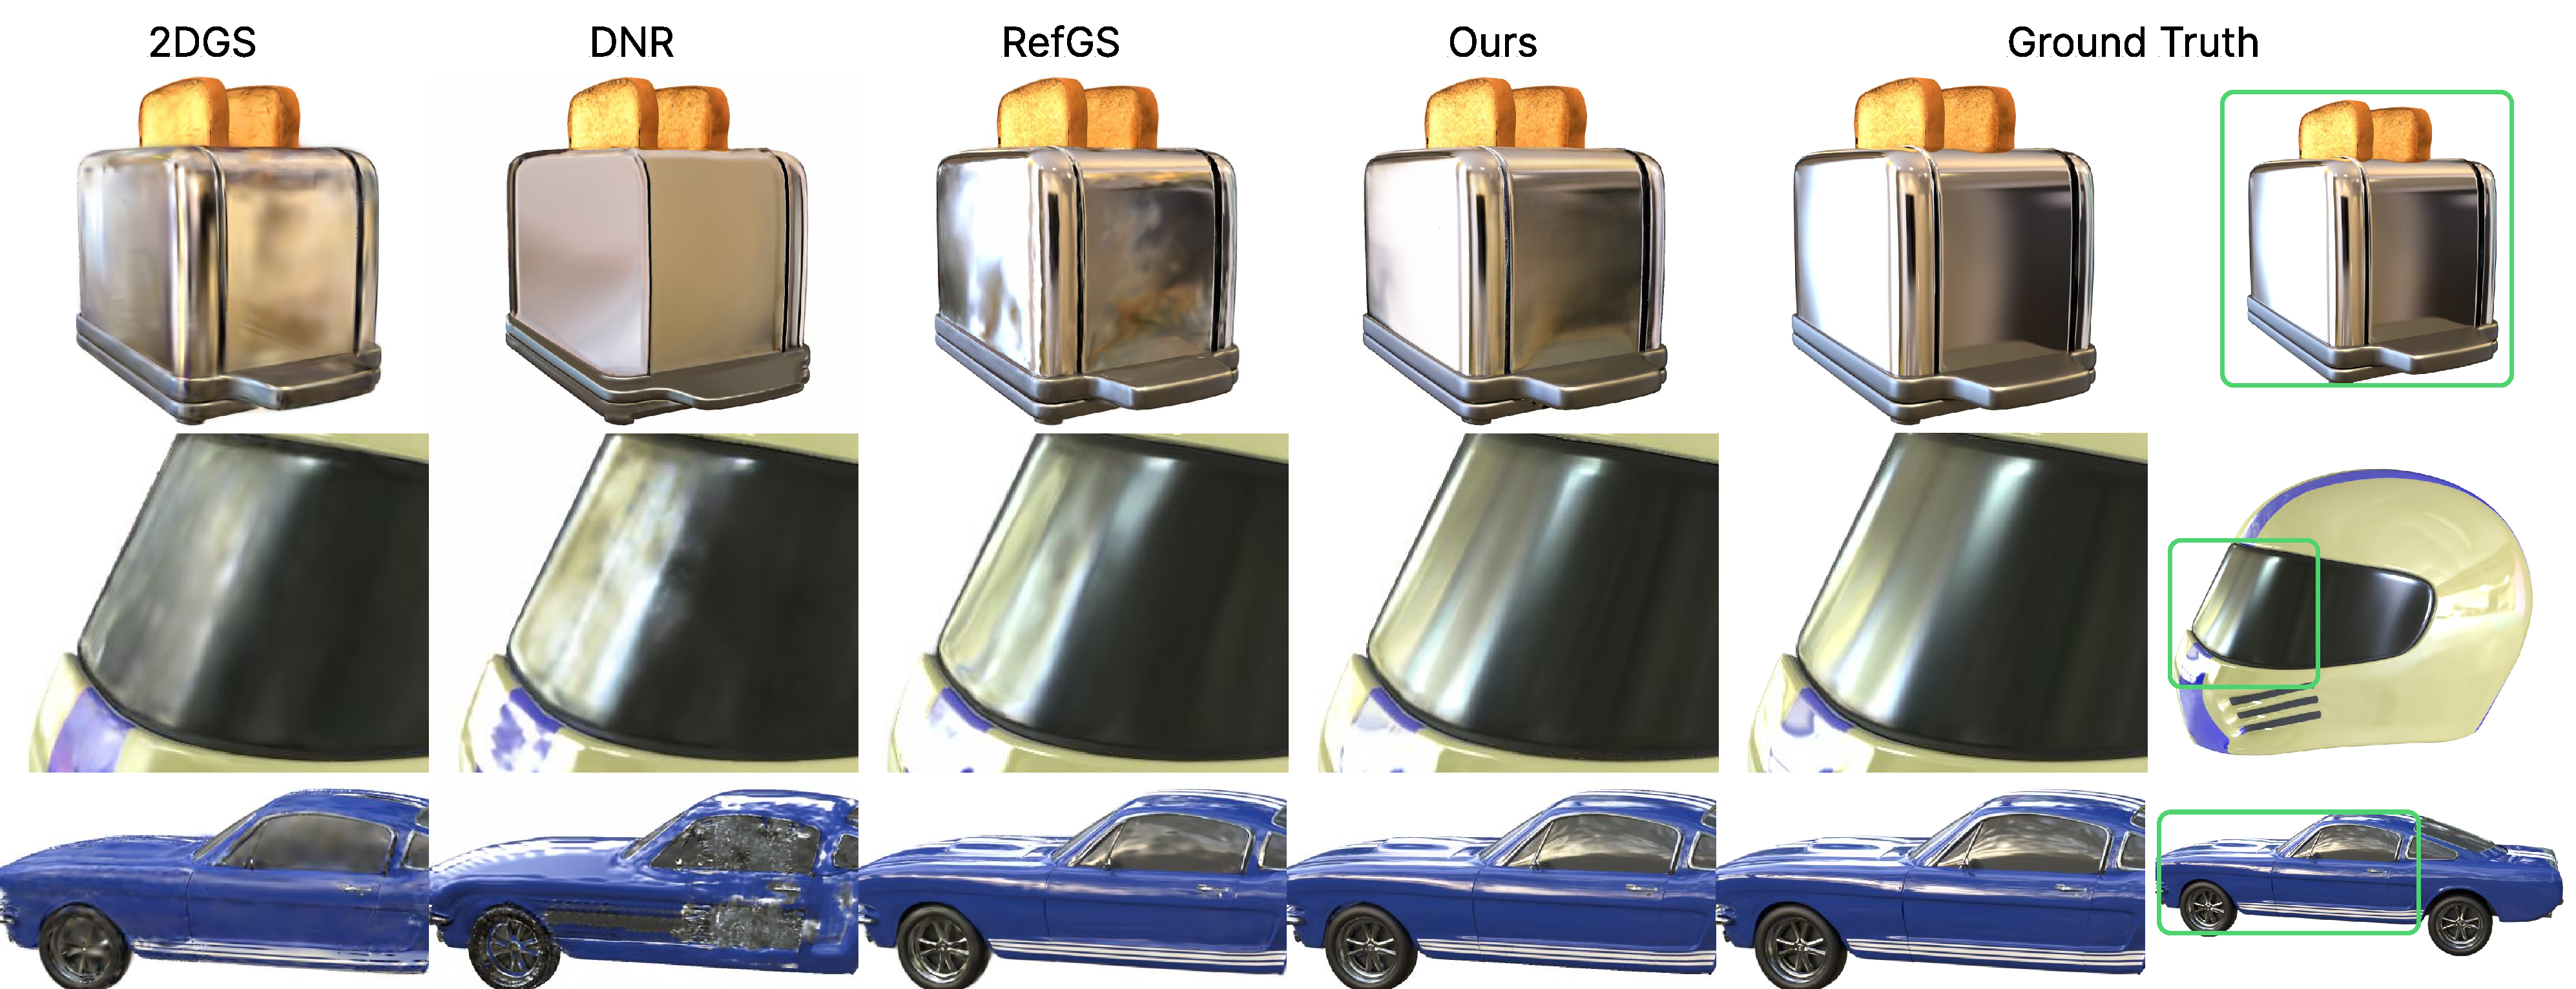
\includegraphics[width=0.95\linewidth]{figs/qualitative.pdf}
    \caption{\textbf{Qualitative comparison on Shiny-Blender.} From left to right: the mesh-constrained baseline 2DGS$^{*}$, DNR, the state-of-the-art RefGS, our method, and ground truth (GT); the rightmost column marks the magnified region on the full object. Our renders reproduce the sharp, high-frequency environment reflections on the metallic surfaces most faithfully; 2DGS$^{*}$ and DNR blur or smear them, RefGS recovers them less crisply.}
    \label{fig:qualitative}
    \vspace{-2mm}
\end{figure}


\subsection{Ablation}
\label{sec:ablation}
Table~\ref{tab:ablation} follows the path by which the appearance model was built. The coplanar
2DGS$^{*}$ baseline suffers the depth-fighting of Sec.~\ref{sec:intro}, and a purely diffuse mixture
cannot represent view-dependent reflection, so both collapse on the reflective scenes. Per-primitive
view-dependent color --- spherical harmonics in 3DGS, or the anisotropic spherical Gaussians of
Spec-Gaussian~\citep{specGaussian} --- is strong for \emph{floating} splats, where overlapping,
depth-ordered primitives compose the appearance. On a single opaque surface that composition is
unavailable: each point takes one order-independent blend, so a per-primitive spherical Gaussian
with an MLP decoder only overfits the sparse views ($34.24$~dB), and dropping it barely changes the
result (Table~\ref{tab:ablation}). The gains come instead from the adaptive hierarchical maps
($+1.2$~dB over a single global map) and from the KAN decoder ($+2.44$~dB over a parameter-matched
MLP).



\subsection{Efficiency}
The full asset ($10^6$ disks, five environment maps, shader) occupies $48.3$ MB on disk. At
$800{\times}800$ we render at $91.7$ FPS on NeRF-Synthetic and $68.6$ FPS on
Shiny-Blender on an NVIDIA H100 (CUDA 12.8), and at $76.8$ FPS on Shiny-Blender on a consumer RTX
4090 (WSL2, Ubuntu 22.04), with a mean CUDA memory footprint of $1.74$ GB (peak $2.75$ GB), all under \texttt{torch.compile}.

% The full asset ($10^6$ disks, five environment maps, shader) occupies $48.3$ MB on disk. At
% $800{\times}800$ we render the test views at $91.7$ FPS on NeRF-Synthetic and $68.6$ FPS on
% Shiny-Blender on an NVIDIA H100 (CUDA 12.8), and at $76.8$ FPS on Shiny-Blender on a consumer RTX
% 4090 (WSL2, Ubuntu 22.04), with a mean CUDA memory footprint of $1.74$ GB (peak $2.75$ GB). All measurements use \texttt{torch.compile}; the H100 figures are from a shared datacenter node.

\subsection{Compaction}
\label{sec:compaction}
Because each disk is an ordinary splat rather than a bespoke primitive, we compact the baked
asset with NanoGS~\citep{nanogs}, a training-free Gaussian-splat simplifier, with no change to our
representation or pipeline. Table~\ref{tab:compaction} reports mean PSNR/SSIM/LPIPS on
Shiny-Blender as we keep 100\%, 50\%, 25\%, and 10\% of the disks: at $10\times$ compaction, mean
PSNR falls by only $2.0$~dB ($38.04\to36.03$), with SSIM and LPIPS degrading similarly gracefully.
Per-scene results (Table~\ref{tab:compaction_perscene}, App.~\ref{app:compaction}) show \emph{teapot} and \emph{ball} essentially unaffected even at $10\times$, while the more detailed \emph{helmet} loses the most. Because compaction reuses tooling built for the Gaussian-splatting community rather than a bespoke method, our representation is compatible with that ecosystem by construction.
\begin{table*}[t]
\centering
\footnotesize
\setlength{\tabcolsep}{3pt}
\begin{minipage}[t]{0.48\textwidth}
\centering
\caption{\textbf{Ablation on Shiny-Blender} along our development path (dataset means;
\textbf{best} in bold). From the 2DGS$^{*}$ baseline we place the mixture on the manifold (2D GMM),
add a per-primitive spherical-Gaussian (SG) reflection with an MLP decoder, drop SG, add our
adaptive hierarchical environment maps (AdaMap), and finally replace the MLP with our KAN. The MLP
and KAN decoders are matched in parameter count.}
\label{tab:ablation}
\begin{tabular}{@{}lccc@{}}
\toprule
Variant & PSNR$\uparrow$ & SSIM$\uparrow$ & LPIPS$\downarrow$ \\
\midrule
2DGS$^{*}$ (baseline) & 27.70 & 0.930 & 0.078 \\
\quad 2D GMM          & 31.40 & 0.952 & 0.057 \\
\quad + SG + MLP      & 34.24 & 0.961 & 0.051 \\
\quad + MLP           & 34.37 & 0.963 & 0.049 \\
\quad + MLP + AdaMap  & 35.60 & 0.971 & 0.038 \\
\quad + KAN + AdaMap  & \textbf{36.99} & \textbf{0.978} & \textbf{0.033} \\
\bottomrule
\end{tabular}
\end{minipage}
\hfill
\begin{minipage}[t]{0.48\textwidth}
\centering
\caption{\textbf{Mesh refinement.} Geometric Metrics Means over the six Shiny-Blender scenes, from Ref-GS
TSDF extractions, without $\rightarrow$ with refinement. MAE$_\text{face}$ refers to face normals of the optimized mesh while MAE$_\text{vert}$  refers to the per-vertex normals of the mesh. We compare against 200 test view normals in ShinyBlender in ray-splat space. Accuracy on a 3d per-point basis with the ground truth mesh is reported. PSNR is a control, not
a result: it confirms the geometry gains are not obtained by trading image quality. These runs use a
single environment map, so absolute PSNR is below Table~\ref{tab:main}. Per-scene results in
App.~\ref{app:refinement}.}
\label{tab:refinement}
% \begin{tabular}{@{}lcc@{}}
% \toprule
% & w/o $\rightarrow$ w/ & $\Delta$ \\
% \midrule
% VN Normal MAE ($^\circ$)$\downarrow$    & $6.31 \rightarrow 5.41$     & $-14.2\%$ \\
% FN MAE ($^\circ$)$\downarrow$    & $7.20 \rightarrow 5.88$     & $-18.3\%$ \\
% CD $\downarrow$                  & $16.200 \rightarrow 15.889$ & $-2.3\%$  \\
% \midrule
% PSNR $\uparrow$ \emph{(control)} & $27.41 \rightarrow 27.86$   & $+0.45$ db   \\
% \bottomrule
% \end{tabular}
\begin{tabular}{@{}lcc@{}}
\toprule
& w/o $\rightarrow$ w/ & Improvement \\
\midrule
MAE$_\text{face}$ ($^\circ$)$\downarrow$ & $7.20 \rightarrow 5.88$ & $+18.3\%$ \\
MAE$_\text{vert}$ ($^\circ$)$\downarrow$ & $6.31 \rightarrow 5.41$ & $+14.2\%$ \\
Acc.\ ($\times10^{-3}$)$\downarrow$      & $5.80 \rightarrow 5.47$ & $+5.7\%$  \\
\midrule
PSNR (dB)$\uparrow$ \emph{(control)}     & $27.41 \rightarrow 27.86$ & $+0.45$ \\
\bottomrule
\end{tabular}

\end{minipage}
\vspace{-2mm}
\end{table*}